\documentclass[11pt]{article}

\usepackage[margin=1in]{geometry}
\usepackage{amsmath,amssymb,amsthm,mathtools}
\usepackage{booktabs,tabularx,array}
\usepackage{graphicx}
\usepackage{microtype}
\usepackage{enumitem}
\usepackage{xcolor}
\usepackage{xurl}
\usepackage[hidelinks]{hyperref}

\definecolor{kernelcolor}{RGB}{0,92,74}
\definecolor{humanproofcolor}{RGB}{45,76,135}
\definecolor{opencolor}{RGB}{145,76,0}
\definecolor{classicalcolor}{RGB}{75,75,75}
\newcommand{\Kernel}{\textcolor{kernelcolor}{\textsc{Kernel}}}
\newcommand{\Human}{\textcolor{humanproofcolor}{\textsc{Proof}}}
\newcommand{\Open}{\textcolor{opencolor}{\textsc{Open}}}
\newcommand{\Classical}{\textcolor{classicalcolor}{\textsc{Classical}}}
\newcommand{\NewResult}{\textsc{New}}
\newcommand{\Realization}{\textsc{Realization}}
\newcommand{\NoGo}{\textsc{No-Go}}

\newcommand{\ii}{\mathrm{i}}
\newcommand{\tr}{\operatorname{tr}}
\newcommand{\rank}{\operatorname{rank}}
\newcommand{\diag}{\operatorname{diag}}
\newcommand{\C}{\mathbb{C}}
\newcommand{\R}{\mathbb{R}}
\newcommand{\id}{\mathbf{1}}
\newcommand{\norm}[1]{\left\lVert #1\right\rVert}

\newtheorem{theorem}{Theorem}[section]
\newtheorem{proposition}[theorem]{Proposition}
\newtheorem{corollary}[theorem]{Corollary}
\newtheorem{definition}[theorem]{Definition}
\newtheorem{remark}[theorem]{Remark}
\newtheorem{conjecture}[theorem]{Conjecture}

\graphicspath{{Sources/figures/}{figures/}}

\title{Null-Spinor Area as the Rest Gap of an Exactly Unitary Dirac Walk\\
\large A Machine-Verified Finite Construction}
% RELEASE GATE: replace the project author line with named authors,
% affiliations, ORCIDs, and a contribution statement before circulation.
\author{Mark Schwab}
\date{July 10, 2026}

\begin{document}
\maketitle

\begin{abstract}
Mass is normally an input to a Dirac quantum walk.  Here it is an output of
null-spinor geometry.  For massless rank-one momenta
$P=\sum_i\psi_i\psi_i^\dagger$, we prove
\[
  \mu^2:=\det P
  =\sum_{i<j}|\psi_i\wedge\psi_j|^2
\]
and $\mu=0$ exactly when the occupied null directions are collinear.  For two
spinors, $z=\psi_1\wedge\psi_2$ canonically defines the odd Hermitian operator
\[
  B_z=\begin{pmatrix}0&z\\ \overline z&0\end{pmatrix},
  \qquad B_z^2=\det(P)\id,
  \qquad (k\sigma_z+B_z)^2=(k^2+\det P)\id.
\]
Thus the positive rest gap is the null-spinor area, with no independent mass
parameter.  Exponentiating $B_z$ gives an exactly unitary walk whose finite
history expansion has turn ratio $-\ii\tan(a\mu)$ and whose quasienergy obeys
$\cos(\omega a)=\cos(ka)\cos(\mu a)$.  We prove a uniform bounded-momentum
$O(1/n)$ many-step limit to Dirac evolution.  In $3+1$ dimensions an arbitrary
position-dependent complex Pluecker field generates an exactly reversible
finite-torus walk with a strict one-cycle causal cone.  Site-dependent chiral
rotation produces explicit endpoint links, while a constant phase produces
none; the complex orientation also appears directly in the finite history
sum through the distinct directed weights $z$ and $\bar z$.  Iterated vector-valued
 Plancherel gives an exact $N^{-3}$ position-space energy normalization for
 nontrivial finite tori, and compactly supported momentum-space spinors inherit
 measure-theoretic $L^2$ convergence.  A high-symmetry audit finds three additional
 zero-quasienergy corner aliases in the massless cubic regulator.  More
 decisively, at body-center momentum the massive step has explicit nonzero
 eigenmodes with eigenvalues $+1$ and $-1$ for every mass angle.  The present
 regulator therefore cannot open a global Floquet gap.  This rules out a
 no-doubling claim and supplies an exact design target.  We also prove that a
 naive degree-one nearest-neighbor repair cannot work: normalization at $q=0$,
 exact all-momentum unitarity, and the full involutory Dirac tangent force its
 stationary amplitude to vanish and force all three even-parity corners to
 equal the origin after any momentum-independent mass coin.  Exact two-step
 blocking closes the mass-only subgroup but not the ordered split family, and
 the positive homogeneous Pluecker action provably selects only the collapsed
 zero scale.  A pre-registered high-momentum benchmark passes all alias,
 body-center, Wilson-gap, and negative-control thresholds.  The algebra, dynamics,
 convergence bounds, Fourier
normalization, and negative controls are checked in Lean~4.  The novelty is
the derived rest operator and its verified dynamical chain, not a new
constant-coefficient $1+1$ walk.  A strict alias-free discrete-time successor,
changing-lattice PDE convergence, and interactions remain open; an absolute
mass requires an additional scale-bearing input.
\end{abstract}

\paragraph{How to read the status marks.}
Origin and verification are independent.  \Classical{} identifies established
mathematics formalized here; \NewResult{} identifies a new theorem or
construction; \Realization{} identifies an explicit model.  \Kernel{} means
the stated finite claim is checked by the pinned Lean kernel; \Human{} means a
complete mathematical proof is given here but its dedicated Lean declaration
is pending; \Open{} marks a named unsolved problem.  Physical interpretations
are never promoted by a verification mark.

\section{Introduction: one invariant, one operator, one walk}

The sum of lightlike momenta need not be lightlike.  In the spinor
representation, each future null momentum is a rank-one positive matrix
$\psi\psi^\dagger$.  A collection of such momenta remains on the null boundary
exactly while its spinors occupy one complex direction.  Once two directions
open, their exterior area is nonzero and the sum moves into the timelike
interior.

This familiar geometry contains a sharper operator statement.  The complex
area $z=\psi\wedge\phi$ is not merely a number whose squared modulus happens
to equal mass squared.  It is the off-diagonal entry of a canonical odd
Hermitian operator.  That operator squares to the invariant momentum
determinant, anticommutes with the velocity grading, and therefore supplies the
rest term of a finite Dirac Hamiltonian.  Its exponential is an exact unitary
turn gate.  The same object thus controls quadratic cost, first-order rest
energy, finite-time rotation, and corner amplitudes.

\begin{figure}[t]
\centering
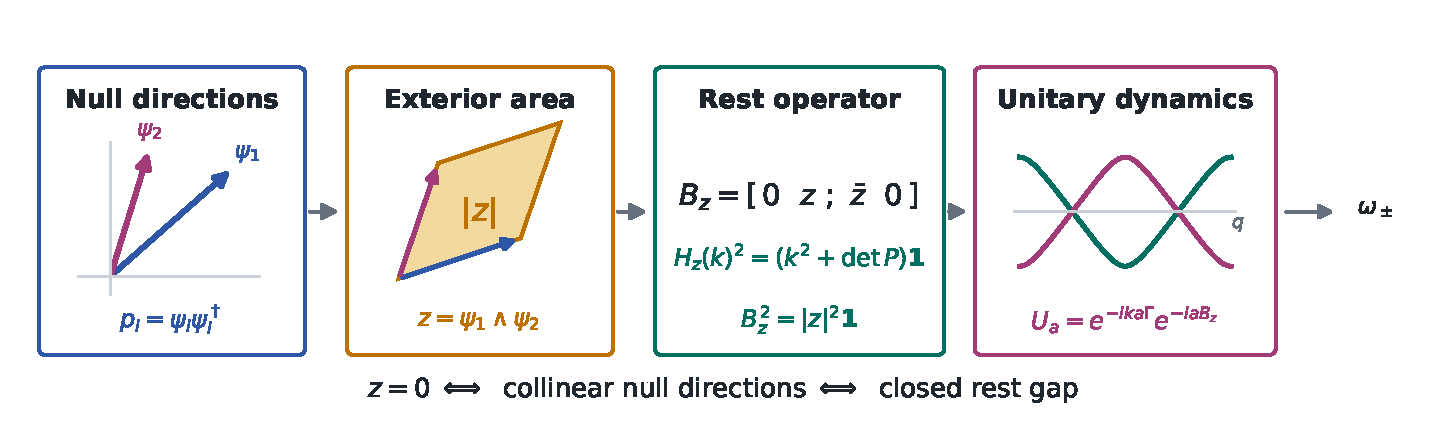
\includegraphics[width=0.98\linewidth]{null_spinor_architecture.pdf}
\caption{The complete finite construction.  The input is a pair of null
spinors, not a preassigned mass angle.  The complex area fixes both the rest
spectrum and the orientation phase of the unitary turn; collinearity is the
exact gap-closing boundary.}
\label{fig:pipeline}
\end{figure}

\begin{center}
\fbox{\begin{minipage}{0.92\linewidth}
\textbf{Synthesis theorem.}
Let $\psi,\phi\in\C^2$, set
$P=\psi\psi^\dagger+\phi\phi^\dagger$,
$z=\psi\wedge\phi$, and $\mu=|z|$.  Then
\[
 \det P=\mu^2,
 \qquad
 B_z=\begin{pmatrix}0&z\\ \overline z&0\end{pmatrix},
 \qquad
 B_z^2=\mu^2\id.
\]
Writing $\Gamma=\diag(1,-1)$ and $H_z(k)=k\Gamma+B_z$, one has
\[
 \Gamma B_z+B_z\Gamma=0,
 \qquad
 \boxed{H_z(k)^2=(k^2+\det P)\id}.
\]
Thus the positive rest energy is $\mu=\sqrt{\det P}$, and the gap closes
exactly on the collinear null boundary.  Multiplying $z$ by a unit phase
changes $B_z$ by unitary conjugation, so the spectrum depends only on $P$ while
the oriented decomposition retains a path phase.  \NewResult{} \Kernel{}
\end{minipage}}
\end{center}

\begin{center}
\fbox{\begin{minipage}{0.92\linewidth}
\textbf{What changes physically, and what does not.}
The Pluecker origin fixes more than a dispersion parameter: it fixes the
complex directed turn amplitudes, their local chiral connection under a
spatially varying field, and the exact gap-closing locus.  It does not by
itself cure lattice aliases or predict an absolute mass.  In fact, within the
four-channel separable degree-one architecture, every even-parity zone corner
is provably locked to the origin after any onsite Pluecker coin; under
the natural positive homogeneous action, every positive configuration has
only the collapsed stationary scale.  These are falsifiable structural
consequences, not interpretive qualifications.  \NewResult{} \Kernel{}
\end{minipage}}
\end{center}

Five contributions organize the paper.
\begin{enumerate}[leftmargin=2em]
  \item We isolate the exterior-area invariant and the exact massless boundary,
  and distinguish the first-order gap $\mu$ from the quadratic invariant
  $\mu^2$.  The Cauchy--Binet identity is classical; its complete finite
  formalization and controls are part of the contribution.
  \item We construct $B_z$ directly from the complex Pluecker coordinate and
  prove the synthesis theorem for arbitrary spinor pairs.  No rational example
  or separately chosen Dirac mass parameter carries the general statement.
  \item We derive the exact unitary turn gate and its corner expansion.  The
  polynomial checkerboard parameter is $\tan(a\mu)$ at finite spacing, not
  $a\mu$ exactly.  A directed-edge path theorem now places $z$ and $\bar z$
  directly in the same finite history sum and proves equality with the actual
  complex Pluecker transfer power.
  \item We give kernel-checked, uniform bounded-momentum many-step estimates
  for the $1+1$ and ordered $3+1$ split-step symbols.  The full complex
  Pluecker phase is covered by unitary conjugacy, not discarded after taking
  its modulus.
  \item We construct an exactly norm-preserving finite-torus $3+1$ local walk
  whose ordered symbol is the product controlled by the $3+1$ estimate.  The
  finite-to-analytic momentum-sign bridge, including its quarter-zone sign, is
  exact.  An iterated three-torus Plancherel theorem gives the exact $N^{-3}$
  wave-packet normalization, and a compact-support multiplier theorem lifts the
  complex walk rate to measure-theoretic $L^2$ convergence.  The full cycle has an explicit two-sided inverse
  and a strict one-shift-per-axis causal cone.  A separate high-symmetry audit
  proves that the massless regulator has three nonzero zero-quasienergy corner
  aliases and that its massive body-center step retains exact $+1$ and $-1$
  modes for every mass angle.  Replacing this globally ungapped regulator and
  proving the infinite-volume PDE limit remain open.  A no-go theorem further
  excludes adding a nonzero stationary coefficient to a degree-one
  nearest-neighbor factor while retaining normalization at the origin, exact
  unitarity, and the full Dirac tangent; its stronger three-axis form proves
  the three even-parity aliases survive every momentum-independent onsite
  coin.  Exact temporal blocking closes the mass subgroup but generates new
  ordered words in the full split family, and a homogeneous-action no-go
  proves that an additional scale-bearing input is required to select
  nonzero $|z|$.
\end{enumerate}

The result sits between spinor-helicity kinematics and discrete relativistic
quantum dynamics \cite{ElvangHuang,ArkaniHamedMassive}.  Cauchy--Binet and the
Pauli map supply the classical foundation.  Feynman's checkerboard and modern
quantum walks show how a massive Dirac propagator can arise from null steps and
direction changes
\cite{FeynmanHibbs,JacobsonSchulman,BisioDarianoTosini,DarianoPathIntegral,MlodinowBrun}.
Our contribution is the exact finite map from the oriented spinor area to the
odd rest operator and then to a controlled unitary walk, together with a
machine-checked dependency boundary.

\subsection*{Nearest constructions and the exact novelty claim}

For constant $z$, the update in this paper is unitarily equivalent to the
standard $1+1$ split-step Dirac walk.  We do not claim otherwise.  What is new
is the input map and its naturality: the coin is generated by the complex
Pluecker coordinate of null momentum factors, its modulus gives the rest
energy, its phase acts by internal conjugacy and survives in oriented turn
amplitudes, and the resulting dependency chain is machine checked.  Table
\ref{tab:comparison} positions that claim against the closest constructions.

\begin{table}[t]
\centering
\scriptsize
\resizebox{\linewidth}{!}{%
\begin{tabular}{@{}lcccccc@{}}
\toprule
Construction & Exact local unitary & Exact finite histories & Mass input
  & Dimension & Continuum control & Machine checked\\
\midrule
Feynman checkerboard \cite{FeynmanHibbs,JacobsonSchulman}
  & not its object & yes & assigned corner weight & $1+1$ & propagator limit & no\\
Dirac QCA \cite{BisioDarianoTosini,DarianoPathIntegral}
  & yes & yes & automaton parameter & $1+1$ & channel/wave-packet bounds & no\\
Split-step DCA \cite{MallickSplitStep}
  & yes & not central & tunable coin angle & $1+1$ & Dirac limit & no\\
Weyl/Dirac QCA \cite{FreeQCA}
  & yes & model dependent & Weyl coupling & up to $3+1$ & relativistic limit & no\\
Tetrahedral Dirac walk \cite{NzonganiTetra}
  & yes & not central & assigned $e^{-\ii\varepsilon m\gamma^0}$ coin
  & $3+1$ tetrahedra & first-order Dirac limit & no\\
This work
  & yes & yes & $z=\psi\wedge\phi$ & $1+1$; finite $3+1$ lift
  & uniform $O(1/n)$ symbols; three-torus $L^2$ & yes\\
\bottomrule
\end{tabular}}
\caption{Structural comparison, not a priority ranking.  The closest QCA
works have stronger field-theoretic or higher-dimensional scope.  The present
distinction is the geometrically generated complex rest operator, the exact
kernel dictionary, and their formal verification.}
\label{tab:comparison}
\end{table}

This comparison also fixes the paper's ceiling.  Its centerpiece is a
one-particle $1+1$ walk with a new geometric input and a rigorous finite chain;
Section~\ref{sec:threeplusone} adds a controlled finite $3+1$ local extension.
It is not yet a new QCA classification, an interacting QCA, or a field theory;
 its exact high-symmetry audit in fact exposes corner aliases and a
 mass-independent body-center no-gap obstruction that a successor regulator
 must remove.

\section{Null-spinor area and the future cone}

\subsection{From rank-one momenta to area}

Let $\psi_1,\ldots,\psi_N\in\C^2$ and define
\begin{equation}\label{eq:momentum}
 M=\begin{bmatrix}\psi_1&\cdots&\psi_N\end{bmatrix},
 \qquad
 P=MM^\dagger=\sum_{i=1}^N\psi_i\psi_i^\dagger.
\end{equation}
Each summand is positive semidefinite and has rank at most one.  Under the
mostly-minus Pauli map, it is a future null four-momentum.  The determinant of
$P$ is the Lorentzian square of the total momentum.

\begin{theorem}[Null-spinor area identity]\label{thm:area}
For the matrix in \eqref{eq:momentum},
\begin{equation}\label{eq:area}
 \det P
 =\norm{\bigwedge{}^2 M}_{\mathrm{HS}}^2
 =\sum_{i<j}\left|\det\begin{bmatrix}\psi_i&\psi_j\end{bmatrix}\right|^2.
\end{equation}
Consequently $\det P\geq0$, and $\det P=0$ if and only if the occupied columns
span a subspace of dimension at most one.
\end{theorem}
\noindent\Classical{} \Kernel{}

\begin{proof}
Cauchy--Binet applied to $MM^\dagger$ expresses its determinant as the sum of
the squared moduli of all $2\times2$ minors of $M$.  Those minors are exactly
the coordinates of $\bigwedge^2M$.  Every summand is nonnegative, so the sum
vanishes exactly when every pairwise wedge vanishes, equivalently when
$\rank M\leq1$.
\end{proof}

Define
\begin{equation}\label{eq:mu}
 \mu:=\norm{\bigwedge{}^2M}_{\mathrm{HS}}=\sqrt{\det P}.
\end{equation}
The quantity $\mu$ is the first-order rest energy; $\mu^2$ is the Lorentzian
quadratic invariant.  The exterior norm makes the geometric word ``area''
literal rather than metaphorical.

For readers who prefer spatial directions, write the null momenta as
$p_i=E_i(1,\mathbf n_i)$ with $E_i\geq0$ and $|\mathbf n_i|=1$.  With the same
mostly-minus normalization,
\begin{equation}\label{eq:angular}
 \mu^2
 =2\sum_{i<j}E_iE_j\bigl(1-\mathbf n_i\mathbin{\cdot}\mathbf n_j\bigr).
\end{equation}
Mass squared is therefore a positive sum of directional disagreements.  It is
zero only when every occupied direction agrees; no cancellation between
different pairs is available.

\subsection{Why the determinant is canonical}

The determinant is not selected merely because it gives the desired answer.
On the physical space of Hermitian $2\times2$ matrices it is the unique real
quadratic form, up to scale, that vanishes on the full rank-one positive
boundary.

\begin{proposition}[Null-boundary uniqueness]\label{prop:unique}
Let $q$ be a real quadratic form on $\operatorname{Herm}(2)$.  If
$q(\psi\psi^\dagger)=0$ for every $\psi\in\C^2$, then
$q(P)=c\det P$ for some $c\in\R$.
\end{proposition}
\noindent\Classical{} \Kernel{}

\begin{proof}
Identify $P\in\operatorname{Herm}(2)$ with $(t,\mathbf x)\in\R^{1,3}$ so that
$\det P=t^2-|\mathbf x|^2$.  Write
$q(t,\mathbf x)=a t^2+2t\,\mathbf b\cdot\mathbf x+\mathbf x^T C\mathbf x$,
with $C$ symmetric.  On the future null cone, homogeneity reduces the
hypothesis to $q(1,\mathbf n)=0$ for every unit vector $\mathbf n$.  Comparing
$\mathbf n$ with $-\mathbf n$ gives $\mathbf b=0$.  Hence
$\mathbf n^TC\mathbf n=-a$ on the unit sphere, which forces $C=-aI$ by
polarization.  Thus $q=a(t^2-|\mathbf x|^2)=a\det P$.
\end{proof}

The Lean theorem uses the four real coordinates of a Hermitian matrix and nine
explicit rank-one spinor probes to eliminate every quadratic coefficient except
one multiple of $pq-r^2-s^2$.  The older real-symmetric slice and a form that
fails the full-boundary hypothesis remain as independent controls.

\begin{corollary}[First-order uniqueness]
Suppose $g$ is nonnegative and homogeneous of degree one on the future cone,
and $g(P)^2$ is a quadratic form vanishing on the rank-one boundary.  Then
$g(P)=c\sqrt{\det P}$ for some $c\geq0$.
\end{corollary}
\noindent\Classical{} \Human{}

This is the logical bridge from a canonical mass-squared invariant to a
canonical rest gap.  The normalization $c=1$ fixes units.

\section{The Pluecker mass operator}

For two spinors, retain the complex orientation data rather than immediately
discarding it into an absolute square:
\begin{equation}
 z:=\psi\wedge\phi=\psi_0\phi_1-\psi_1\phi_0,
 \qquad
 P:=\psi\psi^\dagger+\phi\phi^\dagger.
\end{equation}
Theorem~\ref{thm:area} gives $|z|^2=\det P$.  Define
\begin{equation}\label{eq:Bz}
 B_z:=\begin{pmatrix}0&z\\ \overline z&0\end{pmatrix},
 \qquad
 \Gamma:=\begin{pmatrix}1&0\\0&-1\end{pmatrix}.
\end{equation}

\begin{theorem}[Pluecker-derived rest operator]\label{thm:Bz}
The matrix $B_z$ is Hermitian and odd for the grading $\Gamma$.  More
precisely,
\begin{equation}\label{eq:Bzidentities}
 B_z^\dagger=B_z,
 \qquad
 \Gamma B_z+B_z\Gamma=0,
 \qquad
 B_z^2=|z|^2\id=\det(P)\id.
\end{equation}
For
\begin{equation}\label{eq:Hz}
 H_z(k):=k\Gamma+B_z,
\end{equation}
one has
\begin{equation}\label{eq:hero}
 \boxed{H_z(k)^2=\left(k^2+\det P\right)\id}.
\end{equation}
The rest eigenvalues are $\pm|z|$, and $B_z=0$ exactly when the two nonzero
spinor directions are collinear.
\end{theorem}
\noindent\NewResult{} \Kernel{}

\begin{proof}
Hermiticity is immediate from the two off-diagonal entries.  Direct
multiplication gives
$B_z^2=\diag(z\overline z,\overline z z)=|z|^2\id$, while the diagonal signs
in $\Gamma$ give the anticommutator zero.  Expanding $H_z(k)^2$ leaves
$k^2\id+B_z^2$ because the mixed term vanishes.  Finally $B_z=0$ if and only
if $z=0$, and a two-spinor wedge vanishes exactly on projective collinearity.
Every step of this proof is represented by a general Lean declaration, not by
evaluation of a fixed example.
\end{proof}

Theorem~\ref{thm:Bz} is stronger than assigning the scalar $\det P$ to an
otherwise independent Dirac mass slot.  The odd operator is constructed from
the oriented Pluecker coordinate itself; its square derives the quadratic
invariant.  The distinction between powers is now fixed:

\begin{center}
\begin{tabularx}{0.92\linewidth}{@{}X>{\raggedleft\arraybackslash}p{0.38\linewidth}@{}}
\toprule
Layer & Natural quantity\\
\midrule
Null-spinor kinematics & $\mu^2=\det P=|z|^2$\\
Odd mass operator & $B_z$, with $B_z^2=\mu^2\id$\\
Quadratic costs and Hessians & $\mu^2$\\
Dirac rest energy & $\mu=|z|$\\
Finite unitary turn angle & $a\mu$\\
Exact corner/stay ratio & $\tan(a\mu)$\\
\bottomrule
\end{tabularx}
\end{center}

\subsection{Phase covariance and decomposition independence}

If $u\in\C$ has $|u|=1$, let $W_u=\diag(u,1)$.  Then
\begin{equation}\label{eq:phasecov}
 W_uB_zW_u^\dagger=B_{uz},
 \qquad
 W_uW_u^\dagger=\id.
\end{equation}
Both identities are kernel-checked.  Thus the phase of $z$ rotates the internal
basis but cannot change the rest spectrum.

The construction is also covariant under the spacetime spin group.  If
$A\in\mathrm{SL}(2,\C)$ acts on both spinors by left multiplication, then
\begin{equation}\label{eq:sl2cov}
 (A\psi)\wedge(A\phi)=\det(A)(\psi\wedge\phi)=z,
 \qquad
 B_{(A\psi)\wedge(A\phi)}=B_z.
\end{equation}
This is the algebraic $\mathrm{SL}(2,\C)$ statement covering
proper-orthochronous Lorentz covariance; it is \Kernel{}.  General
$A\in\mathrm{GL}(2,\C)$ acts with the expected determinant weight; that
weighted extension is an algebraic \Human{} corollary, not a separate Lean
declaration in the present development.

\begin{theorem}[Classification of odd Hermitian rest operators]
\label{thm:classification}
Let $B\in M_2(\C)$ be Hermitian and satisfy
$\Gamma B+B\Gamma=0$.  Then there is a unique $w\in\C$ such that
\begin{equation}
 B=B_w=\begin{pmatrix}0&w\\\overline w&0\end{pmatrix},
 \qquad
 B^2=|w|^2\id.
\end{equation}
Consequently the odd Hermitian square roots of $\mu^2\id$ form one phase
circle $w=\mu u$, $|u|=1$, and for $\mu>0$ they are all related by the
conjugacies in \eqref{eq:phasecov}.  Specifying the oriented Pluecker
coordinate $z$ selects one member of that orbit.
\end{theorem}
\noindent\NewResult{} \Kernel{} for the normal form and square;
\Human{} for the phase-orbit corollary.

\begin{proof}
Oddness forces both diagonal entries of $B$ to vanish, and Hermiticity forces
the lower-left entry to be the complex conjugate of the upper-right entry
$w=B_{01}$.  The square is then $|w|^2\id$.  If it equals $\mu^2\id$, then
$|w|=\mu$; for $\mu>0$, write $w=\mu u$ with $|u|=1$ and apply
\eqref{eq:phasecov}.
\end{proof}

This also controls the nonuniqueness of the null decomposition.  If
$M=[\psi\ \phi]$ has full rank and $M'=MR$ with $R\in U(2)$, then
$M'M'^\dagger=MM^\dagger$ and
$\det M'=(\det R)\det M$.  Since $|\det R|=1$, the two mass operators are
related by \eqref{eq:phasecov}.  The unitary-equivalence class of $B_z$ depends
only on $P$; an oriented factorization retains the phase needed by individual
turn amplitudes.  \Classical{} \Kernel{}

The distinction matters physically.  The spectrum is decomposition
independent, while an amplitude can remain sensitive to orientation.  The
construction preserves exactly the information needed by a path sum and
forgets exactly the information a rest energy cannot observe.

\section{Exact unitary null histories}

\subsection{Exponentiating the derived rest term}

For $\mu=|z|>0$, set $\widehat B_z=B_z/\mu$.  Since
$\widehat B_z^2=\id$,
\begin{equation}\label{eq:expB}
 e^{-\ii aB_z}
 =\cos(a\mu)\id-\ii\sin(a\mu)\widehat B_z.
\end{equation}
At $\mu=0$ the expression is understood by continuity and equals $\id$.
Combining the turn with the conditional null translation gives the momentum
symbol
\begin{equation}\label{eq:walk}
 U_a(k;z):=e^{-\ii ak\Gamma}e^{-\ii aB_z}.
\end{equation}
Each factor is unitary.  The two components translate in opposite null
directions; only the odd factor changes direction.

The finite formula in \eqref{eq:expB} is itself closed under composition:
writing it as $C_z(a)$, one has
\begin{equation}
 C_z(a)C_z(a)^\dagger=\id,
 \qquad
 C_z(a)C_z(b)=C_z(a+b).
\end{equation}
The explicit rest eigenvectors, right-unitary decomposition theorem, and this
one-parameter group law are all \Kernel{}.

By phase covariance, $U_a(k;z)$ is unitarily conjugate to the real-mass walk
with parameter $\mu$.  Its determinant is one and its trace is
$2\cos(ka)\cos(\mu a)$.  Therefore an eigenphase $e^{-\ii\omega a}$ obeys
\begin{equation}\label{eq:dispersion}
 \boxed{\cos(\omega a)=\cos(ka)\cos(\mu a)}.
\end{equation}
At $k=0$ the exact eigenphases are $e^{\mp\ii a\mu}$, so the positive
principal-branch quasienergy is $\mu$.  Quasienergy is periodic modulo
$2\pi/a$; no global unbranched equality is asserted.  The real-mass spectral
statement and oriented mass-coin group law are \Kernel{}; the displayed
spectral conjugacy is an immediate corollary of the kernel-checked phase
covariance.

\subsection{The exact corner ratio}

Equation~\eqref{eq:expB} gives two kinds of matrix element.  A component that
keeps its direction contributes $\cos(a\mu)$.  A direction change contributes
$-\ii\sin(a\mu)$ times $z/\mu$ or $\overline z/\mu$, according to its
orientation.  Hence an $n$-step history $h$ with $c(h)$ turns has amplitude
\begin{equation}\label{eq:pathweight}
 A_a(h)
 =e^{\ii\Phi_k(h)}
   \cos(a\mu)^{n-c(h)}
   \bigl(-\ii\sin(a\mu)\bigr)^{c(h)}
   \Xi_z(h),
\end{equation}
where $\Phi_k(h)$ is the translation phase and $\Xi_z(h)$ is a product of
unit-modulus orientation factors.  Whenever $\cos(a\mu)\neq0$,
\begin{equation}\label{eq:tanweight}
 A_a(h)
 =e^{\ii\Phi_k(h)}\cos(a\mu)^n
   \bigl(-\ii\tan(a\mu)\bigr)^{c(h)}\Xi_z(h).
\end{equation}

\begin{proposition}[Unitary checkerboard correspondence]\label{prop:tan}
After removal of the common factor $\cos(a\mu)^n$, the exactly unitary walk is
a corner-weighted checkerboard sum with finite-spacing corner parameter
$\tan(a\mu)$ and the orientation phase inherited from $z$.  Under the opposite
checkerboard sign convention, the parameter changes sign.  In either
convention,
\begin{equation}
 \tan(a\mu)=a\mu+O(a^3),
\end{equation}
but $\tan(a\mu)$ and $a\mu$ are not identical at finite spacing.
\end{proposition}
\noindent\Classical{} for the coin parametrization; \NewResult{} \Kernel{} for
the exact two-weight recursion scaling and the separate transfer-matrix
identification; \NewResult{} \Kernel{} for the directed complex orientation
bookkeeping in the same path sum.

\begin{proof}
Insert the two matrix elements from \eqref{eq:expB} at every time slice.  A
history with $c(h)$ off-diagonal selections and $n-c(h)$ diagonal selections
has exactly the product in \eqref{eq:pathweight}.  Factoring one
$\cos(a\mu)$ from every slice gives \eqref{eq:tanweight}.  The Taylor statement
is the standard expansion of the tangent.
\end{proof}

The Lean development verifies the complete finite dictionary.  Its recursive
two-weight kernel satisfies
\[
 K[s,sw]_n=s^nK[1,w]_n,
\]
and specialization to $s=\cos(a\mu)$ and
$w=-\ii\tan(a\mu)$ gives the unitary checkerboard correspondence exactly when
$\cos(a\mu)\neq0$.  A quarter-angle nondegenerate witness and the
$a\mu=\pi/2$ pure-flip boundary are included.  Separately, the development
verifies that finite null histories weighted by a corner power equal a closed
binomial kernel and satisfy a discrete Dirac recursion, and that the same
direction-resolved history sum equals the corresponding transfer-matrix power.
The direct Gaussian-rational path-sum declaration uses a real mass and corner
weight $+\ii\varepsilon m$ in its stated convention.  Independently, the
directed-edge theorem assigns every history edge the corresponding entry of
the actual complex Pluecker mass coin and proves that the complete oriented
history sum equals its transfer-matrix power.  Thus $\Xi_z$ in
\eqref{eq:pathweight} is now packaged directly: opposite turns carry $z$ and
$\bar z$, with the exact $3+4\ii$ control proving that the two normalized
orientation factors are nonzero and unequal.

The tangent appearance is not asserted as novel by itself.  Exponential and
Euler-angle parametrizations of unitary Dirac-walk coins were related earlier,
including explicit tangent formulas in quantum lattice-Boltzmann work
\cite{SucciQW}.  The contribution here is the exact recursive-kernel scaling
law composed with a coin whose generator is derived from the complex Pluecker
coordinate, together with its machine verification.

\section{Full lattice spectrum, symmetry, and doubling audit}
\label{sec:spectrum}

Quantum-walk claims cannot be judged only at small momentum.  Introduce the
dimensionless variables
\[
 q=ka\in[-\pi,\pi],
 \qquad
 \theta=\mu a,
 \qquad
 \Omega=\omega a.
\]
The Brillouin zone is periodic in $q$, and quasienergy is periodic modulo
$2\pi$.

\begin{theorem}[Complete two-band audit]\label{thm:bands}
The two quasienergy bands are
\begin{equation}\label{eq:bands}
 \Omega_\pm(q)
 =\pm\arccos\!\bigl(\cos q\cos\theta\bigr)
 \pmod{2\pi}.
\end{equation}
They are degenerate only when $q\in\pi\mathbb Z$ and
$\theta\in\pi\mathbb Z$.  On the physical principal branch
$0<|\theta|<\pi/2$, the walk is gapped throughout the Brillouin zone: the
positive rest energy at $q=0$ is $|\theta|/a=\mu$, the interband zero-energy
gap is $2\mu$, and the circular quasienergy gap at the zone edge is also
$2|\theta|$.  At $\theta=0$ there are two massless cones:
\begin{equation}
 (q,\Omega)=(0,0)
 \qquad\text{and}\qquad
 (q,\Omega)=(\pi,\pi).
\end{equation}
For a differentiable band away from a degeneracy,
\begin{equation}\label{eq:groupvelocity}
 v_g=\frac{\partial\omega}{\partial k}
 =\frac{\sin q\cos\theta}{\sin\Omega},
 \qquad |v_g|\leq1,
\end{equation}
with strict inequality for a massive angle whenever the denominator is
nonzero.
\end{theorem}
\noindent\Realization{} \Kernel{} for the trace-derived dispersion, velocity
deficit inequality, exact massless set $\{0,\pi\}$, and uniform massive
discriminant bound; \Human{} for the implicit-differentiation identity in
\eqref{eq:groupvelocity} and for packaging these facts into the displayed
arccos branches.

\begin{proof}
Equation~\eqref{eq:bands} is the principal solution of
\eqref{eq:dispersion}.  A two-band degeneracy requires
$\sin\Omega=0$, equivalently
$|\cos q\cos\theta|=1$.  Each factor has absolute value at most one, so equality
forces $q,\theta\in\pi\mathbb Z$.  At $q=0$ one has
$\Omega_+=|\theta|$ on the stated branch; at $q=\pi$ one has
$\Omega_+=\pi-|\theta|$, whose circular distance to the negative band across
the quasienergy boundary is $2|\theta|$.  Implicit differentiation gives
\eqref{eq:groupvelocity}.  Finally,
\[
 \sin^2\Omega-\sin^2q\cos^2\theta
 =1-\cos^2\theta
 =\sin^2\theta\geq0,
\]
which proves the speed bound and its strict massive form.
\end{proof}

\begin{figure}[t]
\centering
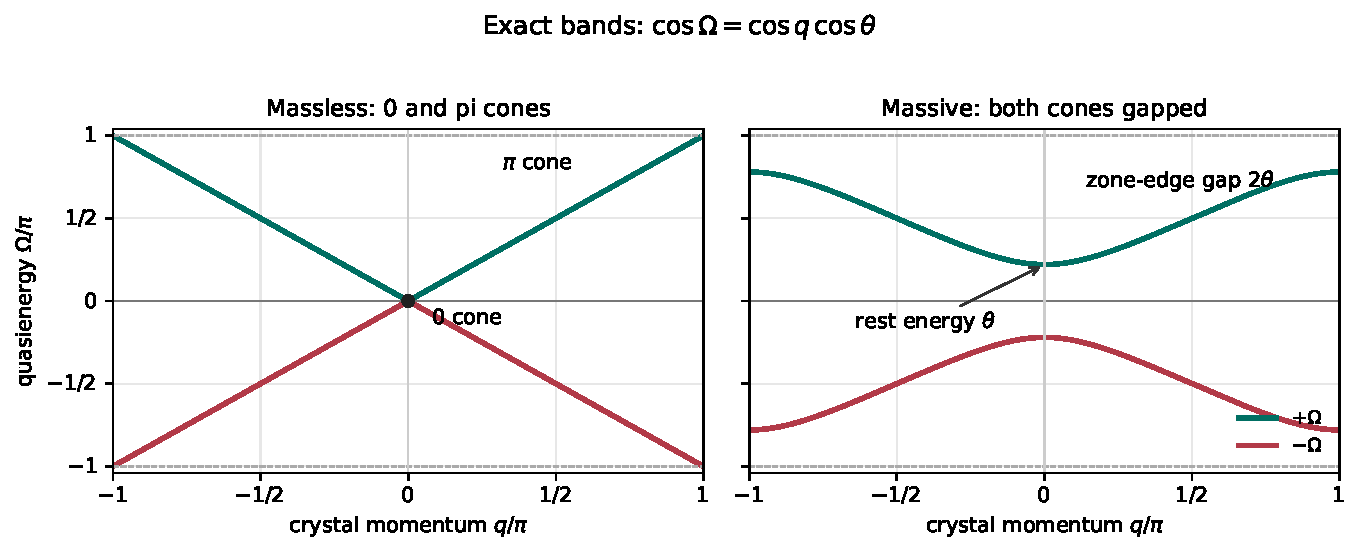
\includegraphics[width=0.92\linewidth]{null_spinor_dirac_bands.pdf}
\caption{Exact quasienergy bands from
$\cos\Omega=\cos q\cos\theta$.  The left panel shows the massless cone at the
origin and its Floquet partner at quasienergy $\pi$.  A nonzero Pluecker area
opens both gaps (right).  The curves evaluate the exact formula; they are not a
fit or numerical simulation.  Generated by
\texttt{Scripts/sim/plot\_null\_spinor\_dirac\_bands.py}.}
\label{fig:bands}
\end{figure}

\paragraph{Doubling and pseudo-doubling verdict.}
The high-momentum $(\pi,\pi)$ cone is a Floquet zone-edge partner of the
low-energy cone.  It is not a second zero-quasienergy root, but it is a second
relativistic band-touching point in the full lattice spectrum.  Following the
terminology of Gupta and Short \cite{GuptaShortDoubling}, it is naturally
classified as a pseudo-doubler: a high-quasienergy mode with a Dirac-like local
dispersion.  The elementary walk therefore does \emph{not} establish a
no-doubling or no-pseudo-doubling theorem.  The bounded
continuum estimate in Section~\ref{sec:continuum} isolates fixed physical
momenta as $a\to0$, sending $q\simeq\pi$ to cutoff momentum; that decoupling is
not the same as removing the finite-lattice partner.

\paragraph{Chiral time frame.}
Let
\[
 U_{\mathrm s}(q,\theta)
 =e^{-\ii\theta\sigma_x/2}
  e^{-\ii q\sigma_z}
  e^{-\ii\theta\sigma_x/2}.
\]
It is unitarily equivalent to $U(q,\theta)$ and obeys the exact chiral relation
\begin{equation}\label{eq:chiral}
 \sigma_yU_{\mathrm s}(q,\theta)\sigma_y
 =U_{\mathrm s}(q,\theta)^\dagger.
\end{equation}
Thus the reciprocal pairing of quasienergies is structural, not an artifact of
the trace calculation.  Equation~\eqref{eq:chiral} is the symmetry statement
used here; a finer antiunitary or Floquet topological classification is left to
a separate analysis \cite{AsbothObuse}.

\paragraph{Robustness.}
If $z$ is perturbed to $z+\delta z$, then
\[
 \bigl||z+\delta z|-|z|\bigr|\leq|\delta z|.
\]
Therefore every perturbation with $|\delta z|<|z|$ remains off the collinear
gap-closing locus and retains a rest energy at least
$|z|-|\delta z|$.  The phase may rotate the internal basis, but by
\eqref{eq:phasecov} it cannot change a constant-coefficient spectrum.

\section{Uniform many-step Dirac control}
\label{sec:continuum}

The finite walk should approximate the continuous Dirac flow over a fixed
macroscopic time, not merely at one infinitesimal step.  For the real
representative of the phase-conjugacy class, write
\begin{equation}
 U(q,r)=e^{-\ii q\sigma_z}e^{-\ii r\sigma_x},
 \qquad
 H(k,\mu)=k\sigma_z+\mu\sigma_x,
 \qquad
 V_t(k,\mu)=e^{-\ii tH(k,\mu)}.
\end{equation}

\begin{theorem}[Uniform bounded-momentum product limit]\label{thm:rate}
For $K,M\geq0$, define
\begin{align}
 C_{\mathrm{box}}(K,M)
   &=2K^2+2M^2+KM^2+K^2M+KM,\\
 D_{\mathrm{box}}(K,M)
   &=4C_{\mathrm{box}}(K,M)
     +4(K+M)^2e^{K+M}.
\end{align}
If $|k|\leq K$, $|\mu|\leq M$, $n>0$, and $|t/n|\leq1$, then
\begin{equation}\label{eq:rate}
 \norm{
   U\!\left(k\frac{t}{n},\mu\frac{t}{n}\right)^n
   -V_t(k,\mu)}
 \leq D_{\mathrm{box}}(K,M)\frac{t^2}{n}.
\end{equation}
The bound is uniform on the displayed parameter box, and its right-hand side
tends to zero as $n\to\infty$.
\end{theorem}
\noindent\NewResult{} \Kernel{}

\begin{proof}[Proof architecture]
The one-step walk differs from $\id-\ii(t/n)H$ by an explicit quadratic
remainder.  The exact exponential differs from the same first-order matrix by
another quadratic remainder, giving
$\norm{U-V_{t/n}}\leq D(k,\mu)t^2/n^2$.  Both matrices are unitary, so the power
telescope has no norm-growth factor:
\[
 \norm{U^n-V_{t/n}^n}\leq n\norm{U-V_{t/n}}.
\]
The exact short-time flows compose to $V_t$, producing the $1/n$ rate.  Finally
$D(k,\mu)\leq D_{\mathrm{box}}(K,M)$ on the parameter box.  Lean checks the
entrywise remainder estimates, operator-norm conversion, unitarity, telescope,
flow composition, box inequality, and limit.
\end{proof}

\begin{figure}[t]
\centering
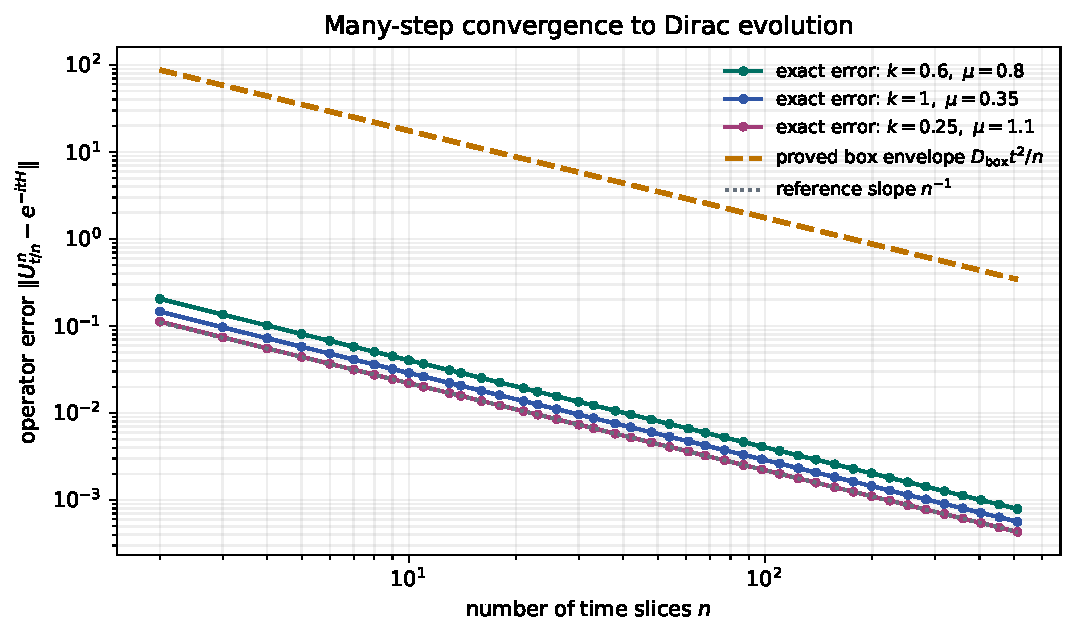
\includegraphics[width=0.88\linewidth]{null_spinor_continuum_rate.pdf}
\caption{Exact many-step operator errors for three nondegenerate parameter
choices.  All follow the proved $n^{-1}$ rate and remain below the explicit
compact-box envelope.  The points evaluate the exact finite matrices; the
envelope and convergence statement are kernel checked.}
\label{fig:continuumrate}
\end{figure}

This proof is a finite-dimensional first-order product-formula argument.  Its
constant is explicit rather than optimized; sharper general Trotter-error
theory provides context for that distinction \cite{ChildsTrotter}.

For $z=\mu u$ with $|u|=1$, the diagonal unitary $W_u$ commutes with $\Gamma$
and conjugates $B_\mu$ to $B_z$.  Unitary invariance of the operator norm
therefore transfers \eqref{eq:rate} to the oriented Pluecker walk.  This
one-line conjugacy corollary is \Human{} pending a combined declaration.

The theorem proves uniform convergence of the finite momentum symbol in
$1+1$ dimensions.  It is not yet an infinite-volume inverse-Fourier theorem,
a position-space PDE convergence theorem, or an interacting limit.  Those
quantifiers are separate problems, not implications hidden in the word
``continuum.''

\section{Finite position kernels and a controlled $3+1$ extension}
\label{sec:threeplusone}

The uniform estimates already imply a finite position-space statement.  Let
$\mathcal K$ be a finite momentum set, let $\chi_x(k)$ be phases with
$|\chi_x(k)|\leq1$, and define the synthesized matrix kernel
\[
 \mathcal S_x[A]:=\sum_{k\in\mathcal K}\chi_x(k)A(k).
\]
Applying the triangle inequality to Theorem~\ref{thm:rate} gives the
kernel-checked bound
\begin{equation}\label{eq:finitefourier}
 \norm{\mathcal S_x[U_n]-\mathcal S_x[V_t]}
 \leq |\mathcal K|D_{\mathrm{box}}(K,M)\frac{t^2}{n}.
\end{equation}
This controls every finite periodic Fourier kernel.  The cardinality factor is
the generic price of applying the triangle inequality pointwise.  It disappears
at the level of normalized $L^2$ wave packets.  For Mathlib's unnormalized
vector-valued transform $\mathcal F$ on $\mathbb Z/N\mathbb Z$, we prove
\begin{equation}\label{eq:plancherel}
 \sum_k
   \norm{(\mathcal F f)(k)}^2
   =N\sum_x
   \norm{f(x)}^2,
 \qquad
 \sum_x
   \norm{\mathcal F^{-1}g(x)}^2
   =\frac1N\sum_k
   \norm{g(k)}^2.
\end{equation}
Consequently, if a modewise error obeys
$\norm{\delta(k)}\leq\varepsilon\norm{c(k)}$, then
\begin{equation}\label{eq:l2wavepacket}
 \sum_x\norm{\mathcal F^{-1}\delta(x)}^2
 \leq \frac{\varepsilon^2}{N}
       \sum_k\norm{c(k)}^2.
\end{equation}
Both identities and the implication are \Classical{} \Kernel{}; a one-mode
packet is included as an exact normalization control.  We also prove the
operator-valued corollary: a uniform bound
$\norm{A(k)-B(k)}\leq\varepsilon$ implies
\eqref{eq:l2wavepacket} for
  $\delta(k)=(A(k)-B(k))c(k)$.  Applying that corollary to the local walk
  uses the exact plane-wave block stated below.  Iterating the transform in
  the three coordinates gives, for $N\geq1$, the kernel-checked product-torus identity
  \begin{equation}\label{eq:plancherel3}
    \sum_{x\in(\mathbb Z/N\mathbb Z)^3}
      \norm{\mathcal F_3^{-1}g(x)}^2
    =\frac{1}{N^3}
      \sum_{k\in(\mathbb Z/N\mathbb Z)^3}\norm{g(k)}^2.
  \end{equation}
  Hence, again for $N\geq1$, a uniform modewise operator error $\varepsilon$ gives the exact
  wave-packet coefficient $\varepsilon^2/N^3$, with no cardinality loss.  The
  momentum-sign bridge is also kernel-checked: for the positive-exponential
  convention the finite character block equals the analytic block at
  $k_j\varepsilon=-2\pi n_j/L$, including an exact quarter-zone $-\ii$ sign
  control.

  There is also a countable successor to the finite Plancherel statement.  If
  $e_n(k)$ is a countable family of mode errors such that
  $e_n(k)\to0$ for every $k$ and
  $\norm{e_n(k)}^2\leq b(k)$ for one summable envelope $b$, then
  \begin{equation}\label{eq:countablel2}
    \sum_k \norm{e_n(k)}^2\longrightarrow0.
  \end{equation}
  This is a direct vector-valued Tannery specialization, proved in Lean with a
  nonzero one-mode control.  It isolates the remaining physical obligation:
  construct the walk-specific square-summable envelope and identify the
  limiting multiplier with the Dirac PDE propagator under a continuum Fourier
  isometry.

  The corresponding measure-theoretic multiplier step is also closed.  If
  $f\in L^2$ and pointwise errors satisfy
  $\norm{e_n(k)}\leq\varepsilon_n\norm{f(k)}$ almost everywhere, where
  $0\leq\varepsilon_n$ and $\varepsilon_n\to0$, then
  \begin{equation}\label{eq:continuousl2multiplier}
    \norm{e_n}_{L^2}\longrightarrow0.
  \end{equation}
  The proof is a kernel-checked `eLpNorm` monotonicity-and-squeeze argument.
  The walk-specific compact-support application is now closed as well.  For any
  fixed $t\in\mathbb R$, suppose $f\in L^2$ and, almost everywhere on the support of $f$,
  $|k_x|,|k_y|,|k_z|\leq K$ and $|z|\leq M$, with $K,M\geq0$.  Applying the
  complex split symbol for $n+1$ steps gives an error multiplier $E_n$ satisfying
  \begin{equation}\label{eq:walkcompactl2}
    \norm{E_nf}_{L^2}\longrightarrow0,
    \qquad
    \norm{E_n(k)f(k)}
      \leq\frac{D_{K,M}t^2}{n+1}\norm{f(k)}.
  \end{equation}
  The displayed pointwise envelope holds for all sufficiently large $n$; the
  finite prefix is irrelevant to the sequence limit.
  This walk-specific composition is \NewResult{} \Kernel{}.  What remains is
  the lattice/continuum Fourier-isometry and identification of the limiting
  multiplier with the position-space Dirac PDE, not compact-support multiplier
  convergence.

The same architecture extends to four internal components.  Let Hermitian
matrices $\alpha_1,\alpha_2,\alpha_3,\beta\in M_4(\C)$ satisfy
\[
 \alpha_i^2=\beta^2=\id,
 \qquad \{\alpha_i,\alpha_j\}=0\ (i\neq j),
 \qquad \{\alpha_i,\beta\}=0,
\]
and set
\[
 H_4(\mathbf k,m)=\sum_{j=1}^3k_j\alpha_j+m\beta.
\]
The explicit matrices used in the artifact obey
\begin{equation}\label{eq:H4square}
 H_4(\mathbf k,m)^2=(|\mathbf k|^2+m^2)\id.
\end{equation}
For a substep $\varepsilon$, define
\begin{equation}\label{eq:3plus1step}
 U^{(4)}_\varepsilon(\mathbf k,m)
 =e^{-\ii\varepsilon k_x\alpha_1}
  e^{-\ii\varepsilon k_y\alpha_2}
  e^{-\ii\varepsilon k_z\alpha_3}
  e^{-\ii\varepsilon m\beta}.
\end{equation}
The order in \eqref{eq:3plus1step} is not cosmetic: the spatial generators do
not commute, and the artifact contains that noncommutation as a negative
control against a false second-order claim.

\begin{theorem}[Finite local $3+1$ walk and compact rate]
\label{thm:3plus1rate}
On a finite periodic three-dimensional position register, there is an explicit
successive-axis update built from one-site conditional shifts and the mass coin
in \eqref{eq:3plus1step}.  It preserves the finite inner product exactly, has
an explicit two-sided inverse, and reads only sites reached by one conditional
source shift along each axis in one cycle.  Its product plane-wave sectors are
invariant, and on each sector the update is
exactly the ordered axis-$0$/axis-$1$/axis-$2$/mass matrix block built from
finite roots of unity.  For the positive-exponential plane-wave convention,
that block is \eqref{eq:3plus1step} when
\begin{equation}\label{eq:latticemomentum}
 k_j\varepsilon=-\frac{2\pi n_j}{L}.
\end{equation}
If
$|k_x|,|k_y|,|k_z|\leq K$, $|m|\leq M$, $n>0$, and $|t/n|\leq1$, then
\begin{equation}\label{eq:3plus1ratebound}
 \norm{\left(U^{(4)}_{t/n}(\mathbf k,m)\right)^n
       -e^{-\ii tH_4(\mathbf k,m)}}
 \leq 16(3K+M)^2e^{3K+M}\frac{t^2}{n}.
\end{equation}
Every finite Fourier synthesis obeys the same bound multiplied by its number
of modes, while the normalized product-torus $L^2$ wave-packet error obeys
the squared bound divided by $N^3$.  Moreover, let $B_4(z)$ be the
phase-retaining rest operator and let $U^{(4)}_\varepsilon(\mathbf k,z)$ be the
chiral conjugate of the displayed step at $m=|z|$.  Its exact comparison flow
is generated by
\[
 H_4(\mathbf k,z)=\sum_{j=1}^3k_j\alpha_j+B_4(z),
 \qquad
 H_4(\mathbf k,z)^2=(|\mathbf k|^2+|z|^2)\id,
\]
and whenever $|z|\leq M$ it satisfies the same bound
\begin{equation}\label{eq:complex3plus1rate}
 \norm{\left(U^{(4)}_{t/n}(\mathbf k,z)\right)^n
       -e^{-\ii tH_4(\mathbf k,z)}}
 \leq 16(3K+M)^2e^{3K+M}\frac{t^2}{n}.
\end{equation}
\end{theorem}
\noindent\Realization{} \Kernel{} for exact local norm preservation, Clifford
square, finite-character plane-wave block, compact rate, finite synthesis
bound, and the trigonometric/sign conversion
\eqref{eq:latticemomentum} to the analytic symbol; \NewResult{} \Kernel{} for
the complex-phase transfer \eqref{eq:complex3plus1rate} and the iterated
three-torus normalization \eqref{eq:plancherel3}.

\begin{proof}[Proof architecture]
Each $\alpha_j$ has eigenvalues $\pm1$.  An explicit unitary eigenbasis turns
the corresponding diagonal one-site conditional shift into the physical
Clifford factor; composing those shifts with the mass coin proves exact norm
preservation.  Direct substitution into every product plane wave extracts one
unit-modulus character per conditional shift and proves the exact ordered
finite block without an asymptotic argument.  The closed form
$e^{-\ii q\alpha_j}=\cos q\,\id-\ii\sin q\,\alpha_j$ identifies the ordered
analytic matrix symbol after the sign convention in
\eqref{eq:latticemomentum}.  A four-factor quadratic remainder estimate, exact
unitarity, and the unitary power telescope then give
\eqref{eq:3plus1ratebound}.  Applying the finite synthesis theorem gives its
position-kernel corollary.
\end{proof}

For $z\neq0$, the phase transfer is exact.  If $W_z$ is the chiral unitary at
the polar angle of $z$, then
\[
 W_zH_4(\mathbf k,|z|)W_z^\dagger=H_4(\mathbf k,z),
 \qquad
 W_ze^{-\ii tH_4(\mathbf k,|z|)}W_z^\dagger
   =e^{-\ii tH_4(\mathbf k,z)}.
\]
The operator norm cannot increase under this conjugation, so the real-mass
estimate transfers without changing its constant.

\subsection*{The $3+1$ high-symmetry verdict}

The continuum tangent is exactly isotropic:
$H_4(\mathbf k,0)^2=|\mathbf k|^2\id$.  The finite cubic walk is not globally
doubler-free.  At the eight corners
$(q_x,q_y,q_z)\in\{0,\pi\}^3$, its massless symbol is
\begin{equation}\label{eq:cornerparity}
 U^{(4)}(q_x,q_y,q_z,0)=(-1)^{r}\id,
 \qquad
 r=\#\{j:q_j=\pi\}.
\end{equation}
Thus $(\pi,\pi,0)$, $(\pi,0,\pi)$, and $(0,\pi,\pi)$ are distinct momenta
 with exactly the same zero-quasienergy symbol as the origin.  Equation
 \eqref{eq:cornerparity}, all three distinctness witnesses, and radial isotropy
 of the continuum square are \Realization{} \Kernel{}.  This is an actual
 finite-regulator obstruction, not a caveat inferred from a plot.

The massive walk has a stronger interior obstruction.  At body-center momentum
$\mathbf q_B=(\pi/2,\pi/2,\pi/2)$, let
$u_\theta=\cos\theta+\ii\sin\theta$ and
\[
 v_+(\theta)=(-u_\theta,0,1,0)^T,
 \qquad
 v_-(\theta)=(u_\theta,0,1,0)^T.
\]
For every real mass angle $\theta$, the exact finite step obeys
\begin{equation}\label{eq:bodycentermodes}
 U^{(4)}(\mathbf q_B,\theta)v_+(\theta)=v_+(\theta),
 \qquad
 U^{(4)}(\mathbf q_B,\theta)v_-(\theta)=-v_-(\theta),
 \qquad v_\pm(\theta)\neq0.
\end{equation}
Equivalently, the body-center step is a non-scalar involution for all
$\theta$.  It therefore retains exact quasienergies $0$ and $\pi$ even after
the mass coin is turned on: the present cubic regulator is globally ungapped.
The closed body-center matrix, involution identity, and both explicit
eigenmodes are \NoGo{} \Kernel{}.

\paragraph{A degree-one stationary-amplitude no-go.}
The most economical proposed repair is to add a stay-put channel to each
nearest-neighbor factor.  The exact ansatz is
\begin{equation}\label{eq:stationarylaurent}
 F(q)=e^{\ii q}A+B+e^{-\ii q}C.
\end{equation}
Let $M$ be any Hermitian involution.  If $F(q)$ is unitary for every real $q$,
$F(0)=\id$, and $F'(0)=-\ii M$, then
\begin{equation}\label{eq:stationarynogo}
 B=0.
\end{equation}
The proof evaluates the exact unitarity residual at $q=\pm\pi/2$; adding the
two resulting matrix identities forces $B^\dagger B=0$.  Specializing
$M=\alpha_j$ rules out a nonzero stationary amplitude in a degree-one factor
with the full Dirac tangent, even before zone-edge separation is imposed.
All three specializations to the live $3+1$ generators are separately
kernel-checked.  This is \NoGo{} \Kernel{}.  A nonvacuity control shows that a partial-channel
Hermitian tangent with a stationary kernel does admit an exactly unitary
degree-one witness with $B\neq0$ and a non-scalar zone edge.  That witness does
not retain the full Dirac tangent.  Thus stationary amplitudes remain viable
only after a genuine change of architecture, such as a larger internal cell,
longer Laurent range, or multistep factorization.

The obstruction is stronger for a separable three-axis product.  Once
$B_x=B_y=B_z=0$, origin normalization forces each factor to obey
$F_j(\pi)=-\id$.  Therefore, for any momentum-independent onsite coin $Q$,
including the complex Pluecker mass coin,
\begin{equation}\label{eq:genericcorneralias}
 U_Q(0,0,0)=U_Q(\pi,\pi,0)=U_Q(\pi,0,\pi)=U_Q(0,\pi,\pi).
\end{equation}
This all-coins alias theorem is \NoGo{} \Kernel{}.  It proves that changing
the onsite mass data cannot repair the cubic partners inside the
four-channel, range-one, single-factor-per-axis architecture.  Extra range,
coupled substeps, or enlarged/ancillary cells are not optional embellishments;
at least one is structurally required.

There is already a constructive Hamiltonian-level route around this no-go.
Using the same live Clifford generators, define
\begin{align}
 M_W(\mathbf q)&=m+r\sum_{j=1}^{3}(1-\cos q_j),\\
 H_W(\mathbf q)&=\sum_{j=1}^{3}\sin q_j\,\alpha_j+M_W(\mathbf q)\beta.
\end{align}
The kernel-checked Wilson identity is
\begin{equation}\label{eq:wilsonsquare}
 H_W(\mathbf q)^2=
 \left(\sum_{j=1}^{3}\sin^2q_j+M_W(\mathbf q)^2\right)\id.
\end{equation}
For $m>0$ and $r\geq0$, the scalar coefficient is bounded below by $m^2$.
For $m=0$ and $r>0$, it vanishes if and only if
$\cos q_1=\cos q_2=\cos q_3=1$; hence all non-origin cubic corners are lifted.
For example, the $(\pi,0,0)$ energy squared is exactly $4r^2$.  This closes
the spectral design problem at the nearest-neighbor Hamiltonian level while
preserving the Dirac tangent.  It does \emph{not} yet close the stricter QCA
problem: $\exp(-\ii tH_W)$ is exactly unitary, but its finite-time exponential
is not asserted to be a finite Laurent polynomial or a strictly finite-range
one-step update.

\paragraph{Exact temporal blocking and nonclosure.}
Define the two-step blocking map by $\mathcal B(U)=U^2$.  The mass-only
Pluecker subgroup closes exactly,
\[
 \mathcal B\bigl(C_z(\varepsilon)\bigr)=C_z(2\varepsilon),
\]
but the ordered spatial split family does not close by doubling its scalar
step.  At the exact $x$--$y$ quarter-turn witness,
\begin{equation}\label{eq:rgcounterexample}
 \mathcal B\bigl(U_{xy}(\pi/2)\bigr)=-\id,
 \qquad U_{xy}(\pi)=\id.
\end{equation}
The smallest multiplicatively closed enlargement is the submonoid generated
by all bare split steps.  These statements are \NewResult{} \Kernel{}: temporal
blocking generates ordered word/coupling data rather than merely a
renormalized copy of the original scalar parameters.  Spatial decimation is a
separate, stronger RG problem.

\paragraph{A proved boundary on scale selection.}
For the finite positive Pluecker action developed here, simultaneous scaling
of both primitive spinors by $t$ gives the exact law
\begin{equation}\label{eq:quarticscalenogo}
 S(t\psi,t\phi;x)=t^4S(\psi,\phi;x).
\end{equation}
Whenever the unscaled action is positive, its radial equation
$4t^3S(\psi,\phi;x)=0$ is equivalent to $t=0$.  The orthogonal-spinor,
positive-quartet control has $S=1/2$, so the obstruction is nonvacuous.
This is \NoGo{} \Kernel{}: the natural positive homogeneous action derives the
curvature associated with a supplied $z$ but cannot spontaneously select a
nonzero $|z|$.  A competing homogeneity, constraint, ensemble scale, or other
dimensionful input must be displayed.
The exact positive control $V_c(t)=(t^2-c)^2$ has stationary points precisely
at $t=0$ or $t^2=c$; for supplied $c=1$, the nonzero points $t=\pm1$ are global
minima.  Selection is therefore possible, but its magnitude is exactly the
new input.  This control is also \Realization{} \Kernel{}.

\paragraph{Pre-registered high-momentum benchmark.}
Before evaluation we fixed $z=3+4\ii$, $\varepsilon=0.2$, Wilson $r=1$, and a
$10^{-10}$ kill threshold.  The oracle then found exactly three non-origin
even-corner aliases (maximum residual $2.30\times10^{-16}$), both body-center
$\pm1$ modes (residuals below $2.24\times10^{-16}$), no non-origin Wilson zero,
and minimum Wilson corner gap $2$.  With $r=0$, all eight corners became
gapless as required by the negative control.  No parameter was fitted.  This
numerical result validates the implementation of the theorem chain; the Lean
identities, not the benchmark, carry the proof.

\begin{figure}[t]
\centering
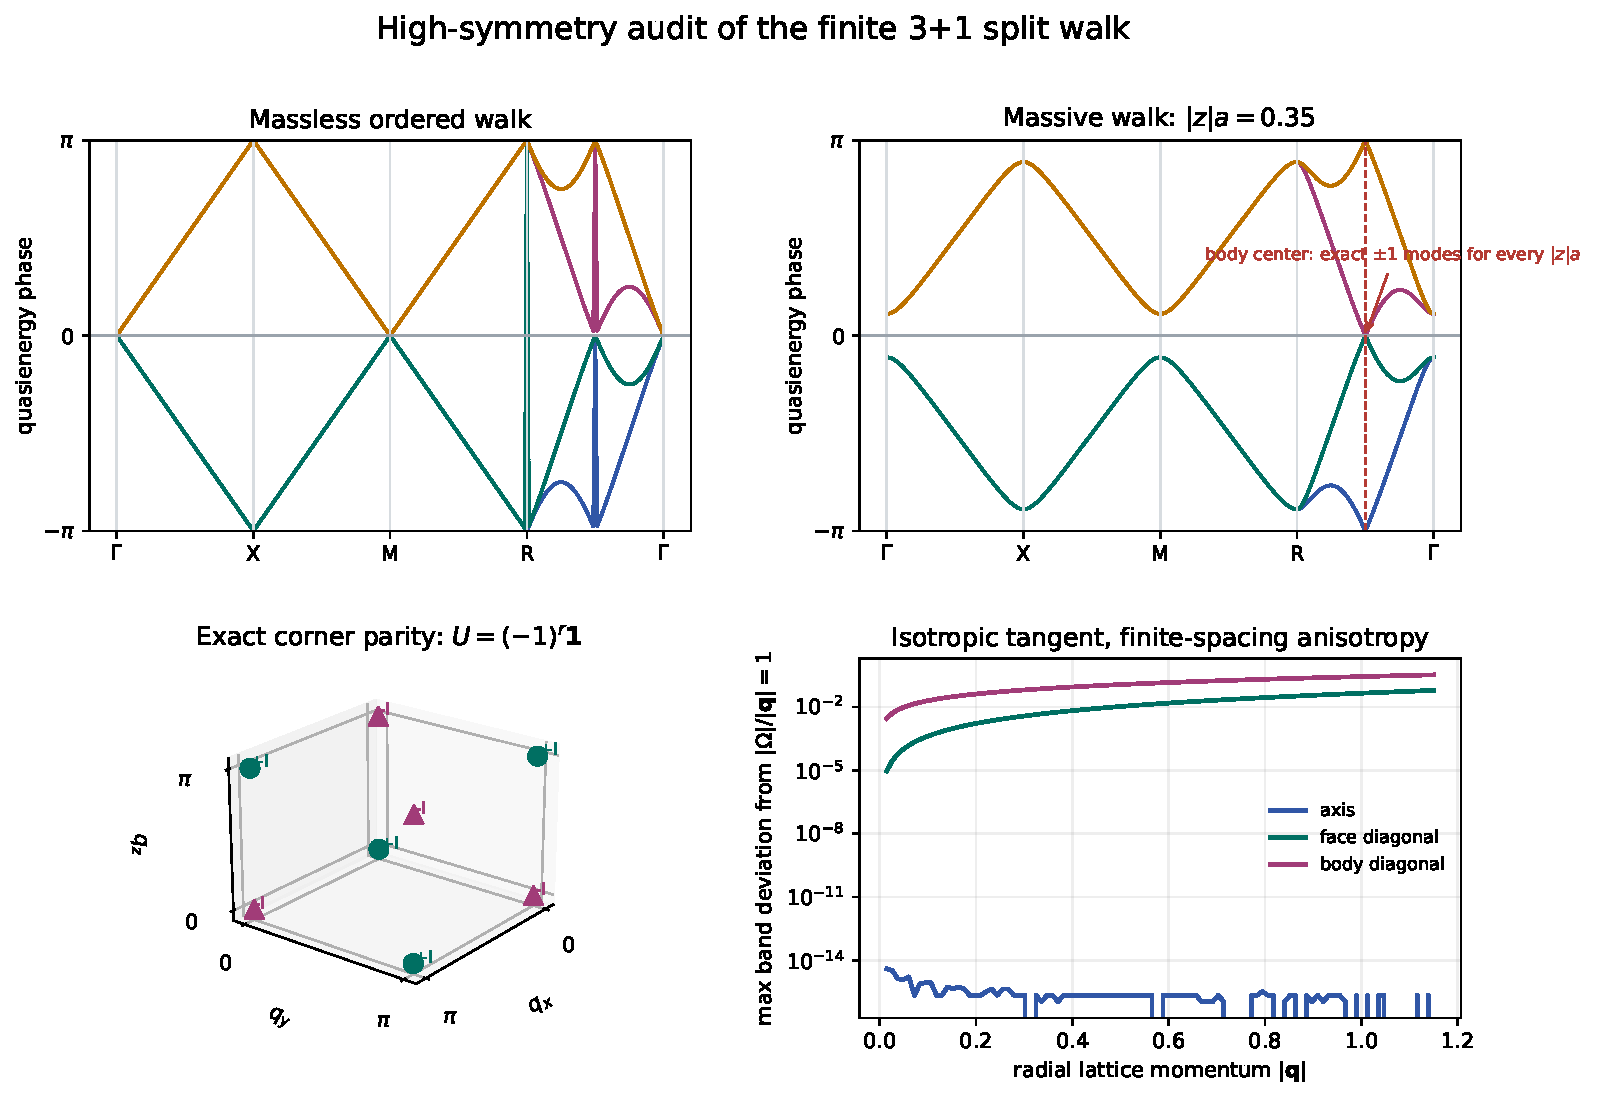
\includegraphics[width=0.98\linewidth]{null_spinor_3plus1_brillouin.pdf}
\caption{High-symmetry audit of the ordered $3+1$ walk.  The small-momentum
tangent is radially isotropic, but the exact massless lattice symbol has four
zero-quasienergy corners: the origin and three even-parity aliases.  The marked
body-center crossing in the massive panel persists for every mass angle by
Eq.~\eqref{eq:bodycentermodes}.  Curves evaluate the exact finite matrices; the
corner classification and body-center eigenmodes are kernel checked.}
\label{fig:3plus1bz}
\end{figure}

\paragraph{Comparison with the tetrahedral walk.}
Nzongani et al.~\cite{NzonganiTetra} place four amplitudes on tetrahedral
facets, compose facet/strict/weakly local shifts with directional coins, and
insert the assigned coin $e^{-\ii\varepsilon m\gamma^0}$; their expansion
recovers the $3+1$ Dirac equation to first order.  Our register and finite
update are different: the present construction is a cubic successive-axis
product with a Pluecker-derived complex mass coin and an explicit many-step
rate.  A constant onsite basis change cannot decide away this difference:
unitary conjugacy preserves equality of symbols at distinct momenta, so every
 constant onsite conjugate of our walk inherits the three aliases above and
 the body-center $\{+1,-1\}$ spectrum.  Any equivalence with a tetrahedral update
 must therefore reproduce those obstructions
or use a non-onsite blocking, changed unit cell, or coarse-graining map.  A
full spectral audit of the tetrahedral symbol is needed before choosing among
those possibilities.

\section{Formal verification and negative controls}

The formal development uses Lean~4.28.0 and Mathlib \cite{Lean4,Mathlib}.  Its
spinor and physics conventions were also cross-checked against the public
PhysLean corpus \cite{PhysLean}.  The trusted
Cauchy--Binet identity lives in the project core; the newer operator and walk
results remain in the draft namespace while their publication interfaces are
reviewed.  Each headline declaration below has a build-enforced assumption
footprint contained in
$\{\mathtt{propext},\mathtt{Classical.choice},\mathtt{Quot.sound}\}$.

\begin{center}
\small
\begin{tabularx}{\linewidth}{@{}p{0.29\linewidth}p{0.15\linewidth}X@{}}
\toprule
Declaration & Status & Mathematical payload\\
\midrule
\texttt{two\_edge\_plucker\_mass\_identity}
 & \Classical{} \Kernel{} & $\det P=|\psi\wedge\phi|^2$\\
\texttt{fin\_bundle\_plucker\_mass\_identity}
 & \Classical{} \Kernel{} & finite-family Cauchy--Binet area sum\\
\texttt{hermitian\_determinant\_uniqueness}
 & \Classical{} \Kernel{} & determinant is the unique quadratic null-boundary form up to scale\\
\texttt{pair\_diracSymbol\_sq}
 & \NewResult{} \Kernel{} & $H_z(k)^2=(k^2+\det P)\id$ for arbitrary pairs\\
\texttt{massOperator\_eq\_zero\_iff\_collinear}
 & \NewResult{} \Kernel{} & exact gap-closing locus\\
\texttt{phase\_covariance}
 & \NewResult{} \Kernel{} & oriented phase acts by conjugacy\\
\texttt{massOperator\_sl2\_invariant}
 & \NewResult{} \Kernel{} & invariance under the defining $\mathrm{SL}(2,\C)$ action\\
\texttt{oddHermitian\_eq\_massOperator}
 & \NewResult{} \Kernel{} & complete normal form for odd Hermitian rest operators\\
\texttt{massCoin\_unitary\_group}
 & \NewResult{} \Kernel{} & exact unitary rest evolution and group law\\
\texttt{unitary\_kernel\_eq\_scaled\_checkerboard}
 & \Realization{} \Kernel{} & exact $\cos^n$ scaling of the two-weight recursion; operator/history identification is supplied by separate transfer-matrix theorems\\
\texttt{exact\_quantum\_walk\_dispersion\_verdict}
 & \Realization{} \Kernel{} & concrete trace identity, trace-to-quasienergy bridge, unitarity, determinant one, and rest eigenphases\\
\texttt{massive\_implies\_subluminal}
 & \Realization{} \Kernel{} & strict full-zone velocity-deficit inequality for massive angle; derivative identity is \Human{}\\
\texttt{massless\_gapless\_classification}
 & \Realization{} \Kernel{} & exact $\{0,\pi\}$ massless band-touching set\\
\texttt{pathAmplitude\_eq\_corner\_power}
 & \Realization{} \Kernel{} & exact real-mass Gaussian-rational corner-power weight; complex orientation is carried by phase conjugacy\\
\texttt{complexPlueckerPathSum\_eq\_transfer\_pow}
 & \NewResult{} \Kernel{} & direct directed-edge history sum using the actual complex coin entries $z$ and $\bar z$\\
\texttt{fixed\_time\_many\_step\_bound}
 & \NewResult{} \Kernel{} & fixed-parameter $D(k,\mu)t^2/n$ estimate\\
\texttt{fixed\_time\_many\_step\_bound\_on\_box}
 & \NewResult{} \Kernel{} & uniform bounded-parameter estimate\\
\texttt{localStep\_preserves\_norm}
 & \Realization{} \Kernel{} & exact finite-torus $3+1$ norm preservation\\
\texttt{inverseSuccessiveWalk\_after}, \texttt{successiveWalk\_after\_inverse}
 & \Realization{} \Kernel{} & explicit two-sided inverse of the complete local cycle\\
\texttt{successiveWalk\_zero\_of\_causalSource\_zero}
 & \Realization{} \Kernel{} & strict one-shift-per-axis causal cone\\
\texttt{Finite3Plus1FourierBridge.localStep\_mode}
 & \Realization{} \Kernel{} & exact finite-character block on every product plane wave\\
\texttt{finiteLocalSymbol\_eq\_analytic\_neg}
 & \Realization{} \Kernel{} & exact finite-to-analytic momentum-sign conversion\\
\texttt{quarter\_zone\_sign\_control}
 & \Realization{} \Kernel{} & nondegenerate $-\ii$ convention fixture\\
\texttt{Pluecker3Plus1ComplexMass.H4\_sq}
 & \NewResult{} \Kernel{} & phase-retaining $3+1$ mass gives $H_4^2=(|\mathbf k|^2+|z|^2)\id$\\
\texttt{complex\_phase\_covariance}
 & \NewResult{} \Kernel{} & chiral covariance of the complex four-component rest operator\\
\texttt{massCoin4\_unitary\_group}
 & \NewResult{} \Kernel{} & derived complex mass coin is unitary with exact group law\\
\texttt{variableComplexLocalStep\_preserves\_norm}
 & \NewResult{} \Kernel{} & arbitrary position-dependent Pluecker profiles, including zero sites, evolve unitarily\\
\texttt{variableComplexLocalStep\_zero\_of\_causalSource\_zero}
 & \NewResult{} \Kernel{} & strict causal cone for the inhomogeneous complex-Pluecker walk\\
\texttt{local\_phase\_connection\_covariance}
 & \NewResult{} \Kernel{} & site-dependent phase induces exact endpoint links and rotates $z(x)$ pointwise\\
\texttt{gaugedCliffordAxisShift\_constant}
 & \NewResult{} \Kernel{} & constant phase produces no endpoint link\\
\texttt{global\_real\_lift\_forces\_zero\_winding}
 & \NoGo{} \Kernel{} & a global real phase lift has zero winding; nonzero index needs branch/transition data\\
\texttt{ComplexPlueckerLocalWalk.complexLocalStep\_mode}
 & \NewResult{} \Kernel{} & phase-retaining mass coin inserted into the exact local Fourier block\\
\texttt{complex\_fixed\_time\_many\_step\_bound\_on\_box}
 & \NewResult{} \Kernel{} & complex Pluecker $3+1$ walk inherits the uniform $O(1/n)$ rate\\
\texttt{complexSplitStep\_eq\_explicit}
 & \NewResult{} \Kernel{} & for $z\neq0$, the conjugacy-defined rate step equals the implemented complex mass-coin product\\
\texttt{localSymbol\_many\_step\_bound\_on\_box}
 & \NewResult{} \Kernel{} & ordered local $3+1$ symbol has uniform $O(1/n)$ rate\\
\texttt{threePlusOne\_finite\_kernel\_bound}
 & \NewResult{} \Kernel{} & finite $3+1$ Fourier-kernel convergence\\
\texttt{dft\_energy}, \texttt{invDFT\_energy}
 & \Classical{} \Kernel{} & exact vector-valued finite Plancherel normalization\\
\texttt{inverseDFT\_wavepacket\_error}
 & \Classical{} \Kernel{} & modewise relative error implies normalized finite $L^2$ control\\
\texttt{inverseDFT\_operator\_wavepacket\_error}
 & \Classical{} \Kernel{} & uniform operator error controls every finite wave packet\\
\texttt{invDFT3\_energy}
 & \Classical{} \Kernel{} & exact inverse-transform energy factor $N^{-3}$ on the three-torus\\
\texttt{inverseDFT3\_operator\_wavepacket\_error}
 & \Classical{} \Kernel{} & exact normalized three-axis operator wave-packet bound\\
\texttt{complex\_walk\_inverseDFT3\_wavepacket\_error\_on\_box}
 & \NewResult{} \Kernel{} & walk-specific complex $3+1$ finite-torus $L^2$ rate\\
\texttt{countable\_l2\_error\_tendsto}
 & \Classical{} \Kernel{} & dominated mode convergence implies countable spectral $L^2$ convergence\\
\texttt{eLpNorm\_two\_tendsto\_zero\_of\_uniform\_relative\_bound}
 & \Classical{} \Kernel{} & uniform relative multiplier error implies measure-theoretic $L^2$ convergence\\
\texttt{walk\_error\_eLpNorm\_tendsto\_zero\_on\_compact\_support\_any\_time}
 & \NewResult{} \Kernel{} & at every fixed time, the complex $3+1$ walk converges in momentum-space $L^2$ on bounded support\\
\texttt{massless\_corner\_parity\_classification}
 & \Realization{} \Kernel{} & exact $\{0,\pi\}^3$ matrix parity classification\\
\texttt{massless\_corner\_quasienergy\_classification}
 & \Realization{} \Kernel{} & exact corner Floquet-quasienergy classification\\
\texttt{origin\_alias\_pi\_pi\_zero}
 & \NoGo{} \Kernel{} & explicit distinct zero-quasienergy corner alias\\
\texttt{body\_center\_walk\_sq}
 & \NoGo{} \Kernel{} & massive body-center step is an involution for every mass angle\\
\texttt{body\_center\_plus\_mode\_eigen},
\texttt{body\_center\_minus\_mode\_eigen}
 & \NoGo{} \Kernel{} & explicit exact $+1$ and $-1$ body-center eigenmodes\\
\texttt{stationary\_forces\_zero}, \texttt{dirac\_no\_go}
 & \NoGo{} \Kernel{} & origin normalization, exact unitarity, and a full involutory tangent exclude a degree-one stationary amplitude\\
\texttt{alpha1/2/3\_stationary\_forces\_zero}
 & \NoGo{} \Kernel{} & the no-go applies to each live $3+1$ axis generator\\
\texttt{live\_degree\_one\_factorized\_lower\_bound}
 & \NoGo{} \Kernel{} & every even-parity corner aliases the origin after any momentum-independent onsite coin\\
\texttt{relaxed\_witness}
 & \Realization{} \Kernel{} & a partial-channel tangent with stationary kernel admits a nonzero stationary amplitude\\
\texttt{WilsonDiracRegulator.H\_sq}
 & \NewResult{} \Kernel{} & exact Wilson--Dirac scalar square in the live Clifford basis\\
\texttt{massless\_energy\_eq\_zero\_iff}
 & \NewResult{} \Kernel{} & positive Wilson parameter removes every non-origin cubic corner at the Hamiltonian level\\
\texttt{bare\_mass\_sq\_le\_energySq}
 & \NewResult{} \Kernel{} & a positive bare mass supplies a uniform global Hamiltonian gap\\
\texttt{no\_constant\_onsite\_equivalence\_of\_corner\_separation}
 & \NoGo{} \Kernel{} & onsite conjugacy cannot erase a corner alias\\
\texttt{massCoin4\_block2\_closes},
\texttt{xy\_blocking\_nonclosure\_control}
 & \NewResult{} \Kernel{} & mass-only temporal blocking closes, while the ordered split family fails exact scalar-parameter closure\\
\texttt{no\_nonzero\_stationary\_scale}
 & \NoGo{} \Kernel{} & the positive quartic Pluecker action selects only the collapsed common scale\\
\bottomrule
\end{tabularx}
\end{center}

The controls are part of the result rather than decorative examples.
\begin{center}
\small
\begin{tabularx}{\linewidth}{@{}p{0.22\linewidth}X X@{}}
\toprule
Claim & Positive/nondegenerate control & Failure or boundary control\\
\midrule
Area creates a gap & standard basis pair gives $z=1$ and $B_z^2=\id$
 & collinear pair $(1,2),(3,6)$ gives $z=0$ and $B_z=0$\\
Full null boundary matters & determinant vanishes on every rank-one edge
 & the form $ac$ vanishes on coordinate rays but fails on the diagonal ray\\
Mass enters at turns & a three-step history is nonzero and mass-dependent
 & at zero mass every positive-corner history vanishes\\
Many-step convergence & rational $(k,\mu)=(3/5,4/5)$ satisfies the bound
 & reversing the mass phase converges to the wrong Hamiltonian numerically\\
$3+1$ factor composition & $(1,2,2,3)$ gives $H_4^2=18\id$ and nonzero norm
 & $\alpha_1\alpha_2\neq\alpha_2\alpha_1$ forbids order erasure and naive second order\\
\bottomrule
\end{tabularx}
\end{center}

The principal verification commands are
\begin{verbatim}
lake env lean PhysicsSM/Draft/NullEdge/PluckerMassOperator.lean
lake env lean PhysicsSM/Draft/NullEdge/PluckerMassDynamics.lean
lake env lean PhysicsSM/Draft/NullEdge/CornerWalkEquivalence.lean
lake env lean PhysicsSM/Draft/NullEdge/FermionDoublingAudit.lean
lake env lean PhysicsSM/Draft/NullEdge/ExactCheckerboardPathSum.lean
lake build PhysicsSM.Draft.NullEdge.ExactQuantumWalkDispersion
lake build PhysicsSM.Draft.NullEdge.FixedMomentumManyStepContinuum
lake build PhysicsSM.Draft.NullEdge.BoundedMomentumManyStepContinuum
lake build PhysicsSM.Draft.NullEdge.Compact3Plus1DiracRate
lake env lean PhysicsSM/Draft/NullEdge/Local3Plus1RateBridge.lean
lake env lean PhysicsSM/Draft/NullEdge/FiniteWalkPositionConvergence.lean
lake env lean PhysicsSM/Draft/NullEdge/FiniteZModPlancherel.lean
lake env lean PhysicsSM/Draft/NullEdge/Finite3Plus1FourierBridge.lean
lake env lean PhysicsSM/Draft/NullEdge/Finite3Plus1AnalyticSignBridge.lean
lake env lean PhysicsSM/Draft/NullEdge/Pluecker3Plus1ComplexMass.lean
lake env lean PhysicsSM/Draft/NullEdge/ComplexPlueckerLocalWalk.lean
lake env lean PhysicsSM/Draft/NullEdge/ComplexPlueckerRateTransfer.lean
lake env lean PhysicsSM/Draft/NullEdge/FiniteTorus3Plancherel.lean
lake env lean PhysicsSM/Draft/NullEdge/FiniteTorus3WalkWavepacket.lean
lake env lean PhysicsSM/Draft/NullEdge/Finite3Plus1BrillouinAudit.lean
lake env lean PhysicsSM/Draft/NullEdge/StationaryAmplitudeNoGo.lean
lake env lean PhysicsSM/Draft/NullEdge/StationaryAmplitudeLiveAxisNoGo.lean
lake env lean PhysicsSM/Draft/NullEdge/FiniteWalkOnsiteEquivalenceObstruction.lean
lake env lean PhysicsSM/Draft/NullEdge/LocalQCAProperties.lean
lake env lean PhysicsSM/Draft/NullEdge/CountableL2WavepacketConvergence.lean
lake env lean PhysicsSM/Draft/NullEdge/ContinuumL2MultiplierBridge.lean
lake env lean PhysicsSM/Draft/NullEdge/CompactSupportL2WalkBridge.lean
lake env lean PhysicsSM/Draft/NullEdge/VariablePlueckerLocalWalk.lean
lake env lean PhysicsSM/Draft/NullEdge/VariablePlueckerPhaseConnection.lean
lake env lean PhysicsSM/Draft/NullEdge/ComplexPlueckerCheckerboardPathSum.lean
lake env lean PhysicsSM/Draft/NullEdge/GlobalPhaseWindingNoGo.lean
lake env lean PhysicsSM/Draft/NullEdge/StrictQCAMinimalArchitecture.lean
lake env lean PhysicsSM/Draft/NullEdge/TemporalBlockingRG.lean
lake env lean PhysicsSM/Draft/NullEdge/Carrier/PluckerScaleSelectionNoGo.lean
lake build PhysicsSM.Draft.NullEdge.OvernightTheoryAxiomGuard
python Scripts/sim/null_edge_regulator_benchmark.py
python Scripts/sim/plot_null_spinor_dirac_bands.py
python Scripts/sim/plot_null_edge_paper_figures.py
\end{verbatim}
The cited modules contain no proof handoff markers or compiled-evaluator proofs.
The working tree is not yet an archival release.  A clean commit, source
archive, theorem ledger, and DOI remain submission requirements.

\subsection*{What mechanization changed}

The formal artifact is scientifically useful only where it improves the
mathematics.  In this development it forced ten corrections that are visible
in the paper.  First, it separated the first-order rest energy $\mu$ from the
quadratic invariant $\mu^2=\det P$ instead of allowing one symbol to drift
between operator orders.  Second, exact unitarity exposed the finite-spacing
corner ratio $\tan(a\mu)$, replacing the tempting but false finite identity
$a\mu=\tan(a\mu)$.  Third, proving an iterated product estimate separated a
one-step Taylor expansion from genuine uniform many-step control.  These are
not the only bookkeeping gains.  Fourth, the exact $3+1$ composition preserved
the noncommuting x/y/z/mass factor order instead of identifying reversed local
 updates.  Fifth, the $1+1$ full-zone audit separated the zero-quasienergy cone
 from its high-quasienergy Floquet partner.  Sixth, the $3+1$ high-symmetry audit
 disproved the tempting global reading of continuum isotropy: the tangent is
 isotropic, three nonzero corners exactly alias the origin, and at body center
 the massive step retains explicit $+1$ and $-1$ modes for every mass angle.
 Seventh, the exact Laurent residual ruled out the most economical proposed
 repair: a nonzero stationary amplitude cannot coexist with origin
 normalization, exact unitarity, and a full involutory tangent inside one
 degree-one nearest-neighbor factor.
 Eighth, the inhomogeneous phase calculation separated a global basis rotation
 from a genuine endpoint connection and proved that a global real lift cannot
 carry nonzero winding.  Ninth, exact temporal blocking showed that the
 mass-only group law closes while the noncommuting spatial split generates a
 larger ordered-word family.  Tenth, the radial derivative of the positive
 Pluecker action proved that its homogeneity collapses rather than selects a
 nonzero scale.
 These are the formalization contributions; the number of declarations is not.

\section{What is forced, derived, realized, and open}

The central scientific distinction is not between bold and cautious language.
It is between different logical verbs.

\begin{center}
\begin{tabularx}{\linewidth}{@{}p{0.16\linewidth}X@{}}
\toprule
Verb & Claim in this paper\\
\midrule
Forced & A quadratic invariant vanishing on the full null boundary is
proportional to the determinant; a nonnegative first-order gap is proportional
to its square root.\\
Derived & The spinor pair gives $z$; $z$ gives $B_z$; $B_z$ gives the Dirac
square, rest gap, unitary turn gate, and orientation-sensitive corner phase.\\
Realized & The split-step null walk exhibits the construction exactly and
converges uniformly on bounded $1+1$ momentum boxes; a finite local $3+1$
 successive-axis walk has an ordered complex-Pluecker symbol with the same
 explicit rate, exact three-torus Plancherel control, and a classified
 high-symmetry failure set.\\
 Open & A walk-specific changing-lattice Fourier/PDE limit, a replacement
 $3+1$ regulator that removes the corner aliases and body-center modes,
 beyond the excluded degree-one stationary-amplitude ansatz, a patched/link
 defect index and localized mode, second quantization, and interactions.\\
\bottomrule
\end{tabularx}
\end{center}

The paper proves a finite free construction.  It does not prove that every
massive particle is composite in the ordinary particle-physics sense.  The
``constituents'' here are null momentum factors of a finite spinor description,
not additional asymptotic particles.  Nor does the theorem compute an absolute
mass scale: rescaling the input spinors rescales $z$ and hence $\mu$.  The
quartic-action no-go sharpens this from an omission to a proved boundary for
the natural positive homogeneous action.

The result does support a precise statement: a timelike rest gap can be encoded
entirely by massless rank-one momentum primitives, and the gap is exactly the
area opened between their spinor directions.  In the derived walk, microscopic
translation occurs along null channels while subluminal drift and a rest gap
arise from coherent direction changes.  This is an exact property of the
finite model, not yet a universal ontology of nature.

\section{Interpretation and open problems}

The larger null-information program studies a four-term finite carrier square,
positive cohomology, closure interactions, and discrete frame data.  Those
structures motivated the present theorem but are not required to prove it.
They belong in a companion paper unless they acquire a theorem that depends on
$B_z$.

The next problems are sharply ordered.
\begin{enumerate}[leftmargin=2em]
  \item \textbf{Complete the lattice-to-PDE identification.}
  The finite product DFT, its exact $N^{-3}$ normalization, and the
  walk-specific compact-support momentum-space $L^2$ limit are closed.  Control
  the changing lattice/continuum Fourier spaces and identify the limiting
  multiplier with the position-space Dirac PDE propagator.  For unrestricted
  data one must additionally construct a global or square-summable envelope.
  Equations \eqref{eq:plancherel3}, \eqref{eq:countablel2},
  \eqref{eq:continuousl2multiplier}, and \eqref{eq:walkcompactl2} close the
  finite, abstract countable, and compact-support multiplier steps, not that
  final physical identification.
  \item \textbf{Remove the lattice partners without losing the derivation.}
  The no-go \eqref{eq:stationarynogo} rules out the naive degree-one
  stationary-amplitude factor with a full Dirac tangent.  The Wilson
  construction \eqref{eq:wilsonsquare} now removes the unwanted corners and
  gives a uniform massive gap for a nearest-neighbor Hamiltonian.  The open
  task is to retain that spectral success in a strictly finite-range,
  exactly unitary discrete-time update.  Test the enlarged
  internal cells, longer Laurent range, or multistep stationary constructions
  motivated by Gupta and Short \cite{GuptaShortDoubling} while preserving the
  Pluecker-derived coin and exact path dictionary.  In $3+1$, remove the three
  proven even-parity origin
   aliases and both mass-independent body-center modes while retaining locality,
   unitarity, continuum isotropy, and the complex-mass rate.  Equations
   \eqref{eq:cornerparity} and \eqref{eq:bodycentermodes} are the regression
   tests.
  \item \textbf{Complete the tetrahedral comparison.}
  Compute the tetrahedral walk's full Bloch symbol in a common blocked unit
  cell and audit its corners, bands, and locality radius.  Constant onsite
  equivalence is already constrained by the alias-preservation no-go; a
  genuine comparison must specify any blocking or coarse-graining map.
  \item \textbf{Generalize the Pluecker rest operator.}
  For larger null families, seek a canonical odd Hermitian operator from
  $w=(\psi_i\wedge\psi_j)_{i<j}$ whose square is the complete area budget and
  whose phase/moduli classification is decomposition-independent.
  \item \textbf{Build patched defects from the local $z$ field.}
  The position-dependent unitary update, its inverse and causal cone, and exact
  site-dependent chiral connection are now closed.  A globally lifted real
  phase has zero winding, so the next theorem must introduce branch/transition
  links or a sign/domain wall through the collinear zero set, reduce that
  operator to a finite index, and exhibit a localized protected mode.  The
  existing finite winding operator is not yet derived from this local field.
  \item \textbf{Derive an interacting shared action.}
  The free operator now generates its square, gap, and exponential.  A complete
  dynamics requires one field-valued action whose reductions produce both the
  null-spinor geometry and the spinor evolution, rather than assigning the
  same parameter to separate models.
  \item \textbf{Add a scale-bearing selection mechanism and derive couplings.}
  The positive homogeneous Pluecker action now has a proved no-go: every
  positive configuration has only the collapsed stationary common scale.
  Therefore a nonzero solution must display a competing homogeneity,
  constraint, ensemble scale, or other dimensionful input and quantify which
  observed scale remains supplied.  Interaction strengths and gauge
  representations remain open.
\end{enumerate}

The finite construction encodes spacetime information algebraically through a
fixed Pauli map and null direction grading.  Emergence of a dynamical continuum
geometry remains conjectural.  We therefore do not claim that the paper starts
without spacetime structure; it starts without primitive timelike motion or a
primitive mass term inside the finite model.

\section{Conclusion}

The result readers should retain is compact.  Null spinors open an exterior
area.  That area is the positive rest gap, its square is the momentum
determinant, and its complex orientation is the off-diagonal part of an odd
Hermitian mass operator.  The collinear null boundary is exactly the
gap-closing locus.

The operator does more than rename a scalar.  It produces the relativistic
Dirac square, exponentiates to the exact unitary turn, and fixes the finite
corner ratio, including the directed $z$/$\bar z$ factors in the exact history
sum.  The associated split-step walk converges uniformly on bounded
$1+1$ momentum boxes at an explicit $O(1/n)$ rate, and its transfer-matrix
history representation has a two-weight recursion that scales to the
checkerboard corner ratio $-\ii\tan(a\mu)$.  The
   finite local $3+1$ extension now accepts arbitrary position-dependent
   Pluecker profiles, preserves norm exactly, has an explicit inverse and
   causal cone, and turns local phase variation into endpoint links.  Its ordered symbol
   with complex-phase compact-box control and exact three-torus Plancherel
   normalization, together with compact-support momentum-space $L^2$
   convergence.  These statements form one finite chain from null geometry to
   rest energy and propagation.  The same audit proves where that chain
   presently stops: the cubic regulator has three exact zero-quasienergy corner
   aliases, and its massive body-center step retains exact $0$ and $\pi$
   quasienergies for every mass angle.  The degree-one stationary-amplitude
   no-go excludes the simplest attempted repair, and its factorized form proves
   that every onsite mass coin leaves all three even-parity aliases intact.
   A Wilson term removes the
   non-origin corners and opens a uniform massive gap at the local-Hamiltonian
   level; converting that success into a strictly finite-range discrete-time
   regulator remains open.  Exact temporal blocking further shows that the
   mass subgroup closes while the full split family generates a larger ordered
   monoid, and the homogeneous-action no-go proves that a nonzero absolute
   mass needs an additional scale-bearing input.

What remains is equally definite: a changing-lattice position-space PDE limit, a local
 strictly finite-range unitary regulator outside the degree-one
 stationary-amplitude no-go that matches the Wilson Hamiltonian's spectral
 success without sacrificing the derived coin, a blocked
 comparison with the tetrahedral construction, a patched defect/index theorem,
 and a second-quantized interacting extension.  Success would extend a machine-verified finite
rest-gap construction into a broader discrete relativistic dynamics.  Failure
at any named step would locate the boundary of the idea rather than dissolve
it into analogy.

\begin{thebibliography}{99}

\bibitem{ElvangHuang}
H.~Elvang and Y.-t.~Huang,
\emph{Scattering Amplitudes}, arXiv:1308.1697.

\bibitem{ArkaniHamedMassive}
N.~Arkani-Hamed, T.-C.~Huang, and Y.-t.~Huang,
\emph{Scattering Amplitudes For All Masses and Spins},
JHEP 11 (2021) 070, arXiv:1709.04891.

\bibitem{FeynmanHibbs}
R.~P.~Feynman and A.~R.~Hibbs,
\emph{Quantum Mechanics and Path Integrals}, McGraw--Hill, 1965.

\bibitem{JacobsonSchulman}
T.~Jacobson and L.~S.~Schulman,
\emph{Quantum stochastics: the passage from a relativistic to a
non-relativistic path integral}, J. Phys. A 17 (1984) 375.

\bibitem{BisioDarianoTosini}
A.~Bisio, G.~M.~D'Ariano, and A.~Tosini,
\emph{Quantum field as a quantum cellular automaton: the Dirac free evolution
in one dimension}, Ann. Phys. 354 (2015) 244, arXiv:1212.2839.

\bibitem{DarianoPathIntegral}
G.~M.~D'Ariano, N.~Mosco, P.~Perinotti, and A.~Tosini,
\emph{Path-integral solution of the one-dimensional Dirac quantum cellular
automaton}, Phys. Lett. A 378 (2014) 3165--3168, arXiv:1406.1021.

\bibitem{MallickSplitStep}
A.~Mallick and C.~M.~Chandrashekar,
\emph{Dirac cellular automaton from split-step quantum walk},
Sci. Rep. 6 (2016) 25779, arXiv:1509.08851.

\bibitem{SucciQW}
S.~Succi, F.~Fillion-Gourdeau, and S.~Palpacelli,
\emph{Quantum lattice Boltzmann is a quantum walk},
EPJ Quantum Technol. 2 (2015) 12.

\bibitem{FreeQCA}
A.~Bisio, G.~M.~D'Ariano, P.~Perinotti, and A.~Tosini,
\emph{Free quantum field theory from quantum cellular automata: Derivation of
Weyl, Dirac and Maxwell quantum cellular automata},
Found. Phys. 46 (2016) 1032--1081, arXiv:1601.04832.

\bibitem{NzonganiTetra}
U.~Nzongani, N.~Eon, I.~Marquez-Martin, A.~Perez, G.~Di Molfetta, and
P.~Arrighi,
\emph{Dirac quantum walk on tetrahedra},
Phys. Rev. A 110 (2024) 042418, arXiv:2404.09840.

\bibitem{AsbothObuse}
J.~K.~Asboth and H.~Obuse,
\emph{Bulk-boundary correspondence for chiral symmetric quantum walks},
Phys. Rev. B 88 (2013) 121406(R), arXiv:1303.1199.

\bibitem{GuptaShortDoubling}
C.~Gupta and A.~J.~Short,
\emph{Fermion doubling in Dirac quantum walks},
Phys. Rev. A, accepted (2026), arXiv:2601.15885,
doi:10.1103/kkz3-fthm.

\bibitem{MlodinowBrun}
L.~Mlodinow and T.~A.~Brun,
\emph{Discrete spacetime, quantum walks, and relativistic wave equations},
Phys. Rev. A 97 (2018) 042131, arXiv:1802.03910.

\bibitem{ChildsTrotter}
A.~M.~Childs, Y.~Su, M.~C.~Tran, N.~Wiebe, and S.~Zhu,
\emph{A theory of Trotter error}, Phys. Rev. X 11 (2021) 011020,
arXiv:1912.08854.

\bibitem{Lean4}
L.~de Moura and S.~Ullrich,
\emph{The Lean 4 theorem prover and programming language},
CADE-28, Lecture Notes in Computer Science 12699 (2021) 625--635.

\bibitem{Mathlib}
The Mathlib Community,
\emph{The Lean mathematical library}, Proceedings of CPP 2020, 367--381.

\bibitem{PhysLean}
J.~Tooby-Smith,
\emph{HepLean: Digitalising high energy physics}, arXiv:2405.08863.

\end{thebibliography}

\end{document}
